\subsection{Introduction}
When a stimulus is provided to the brain, the mostly activated area is always constituted by a network of regions: it's never only the stimulated area.\\
This is because diffusion (or \textbf{volume conduction}) is present inside the brain, and it inflates any connectivity estimates. A lot of attention to this phenomenon must be paid. This because the instantaneous field spread creates spurious connections, that cannot be identified directly looking at numbers, since these correlates can be modeled as a linear combination (even if the brain is not isotropic) of all possible elements in the field across all the channels, and they include also the significant ones.\\
Anyway, volume conduction can be considered as an instantaneous contribution of the field: a single activity from an electrical dipole reaches all the sensors at the same time, and this can be translated in a phase difference equal to 0. 
So, data that has a \textbf{0 lag phase} can be traced back to volume conduction.\\
In order to mitigate this effect, is hence necessary to cancel out all the phase differences whose angle is 0. This can be done in two ways:
\subsubsection{Imaginary PLV (and Imaginary Coherence)} 
\begin{figure}[H]
    \centering
    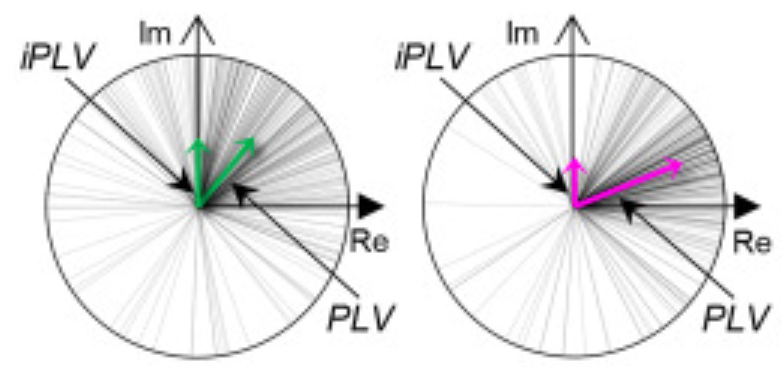
\includegraphics[scale=0.6]{14_1.PNG}
\end{figure}
As already introduced, from the PLV a vector can be obtained as the algebraic sum of all the vectors in the unitary circle. This resultant vector can then be projected onto the real and the imaginary axes. 
In this the instantaneous field spread, given by all those components with phase angles equal to 0, will lie on the real axis. So, they can be completely eliminated just looking at the projection of the PLV on the imaginary axis.
In this way, however, the 0 lag is removed, but a new problem is introduced: every vector that is between \(-45^\circ\) and \(45^\circ\) is underestimated because their contribution weights more on the real axis than on the imaginary one.\\
This formulation allow to distinguish between the contributions due to volume conduction and the ones related to connectivity. However, spurious connectivity can derive also from the fact that neurons are locally connected and two brain regions may be connected through not all the neurons that belong to a narrow ensemble.
The following model can be considered:
\begin{figure}[H]
    \centering
    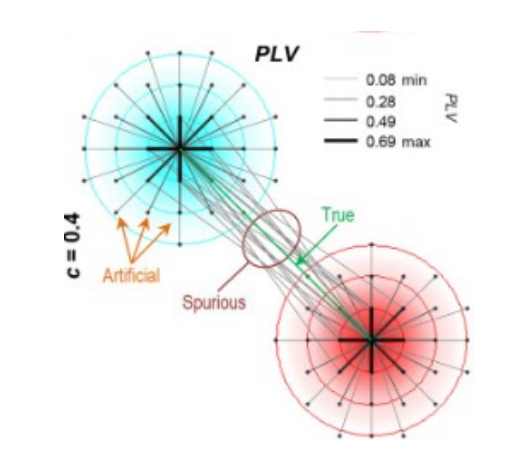
\includegraphics[scale=0.6]{14_2.PNG}
\end{figure}
Two brain regions are composed of many neurons of which just one is linked to the other area. Many electrodes are placed between these two areas and all the neurons in each area are tightly connected together and exchange information.
Since local connectivity is very fast, it can have 0-lag components. Discarding them, also some elements related to physiological activity can be eliminated, so the disadvantage of this approach is also that it can cancel out also real genuine 0-lag values.\\
On the other hand, this approach has the big advantage that its mathematical formulation is the same seen before for PLV, but instead of taking the absolute value of the PLV, the imaginary part and than the absolute value are considered.
\subsubsection{Weighted Phase Lag Index}
This approach is more complex in term of formulation but it has almost the same properties.
\subsection{Assessing Significance}
Independently of the way in which the connectivity profiles are looked at, it's important to understand how to assess the actual significance of the observations that are made.
The best way to do that is using a distribution under the null hypothesis. In the classical tests, it relies on the assumption that data are distributed according to a Gaussian distribution. However, in this case phase angles can't be Gaussian distributed because the statistic is circular, so surrogate statistics need to be built.\\
To do it, a circular rotation of one time series with respect to the other can be used (same of previous lesson): in this way, the auto-correlation of one channel is maintained but the cross-correlation of two different channels is disrupted because of the time rotation. This allow to observe the data under the null hypothesis of no time correlation between different regions.
\subsubsection{Algorithm to test for Significance}
Since the recording is multi channel, connectivity statistics such as PLV or any other pair wise metric can be computed. This will give the weighted \textbf{adjacency matrix}: a matrix in which in each pixel the connectivity between channel \(i\) and \(j\) is represented.
Then the surrogate statistics is calculated and the null distribution is built.
\begin{figure}[H]
    \centering
    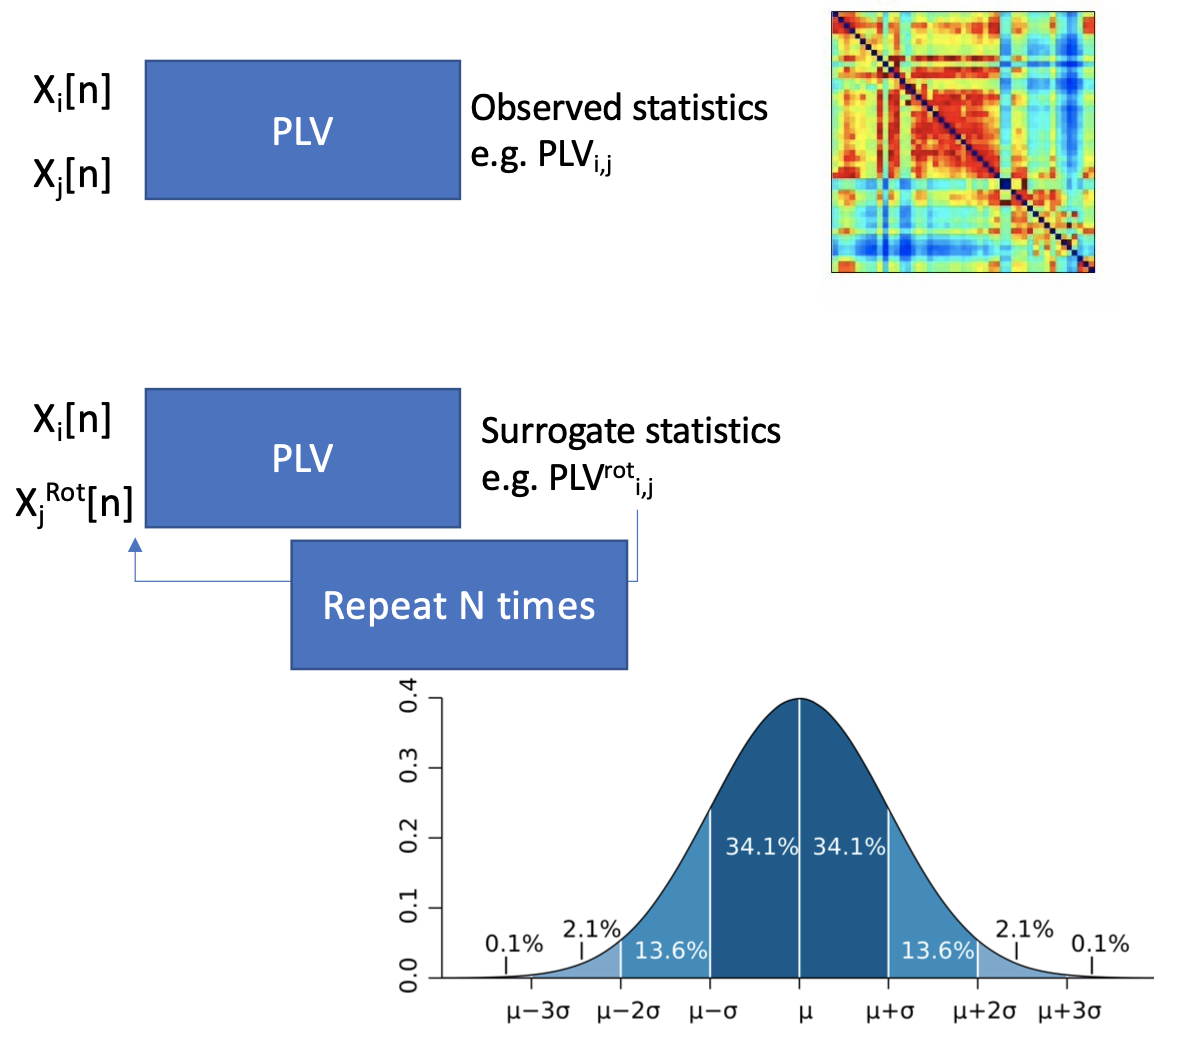
\includegraphics[scale=0.45]{14_3.PNG}
\end{figure}
To do this the statistics is computed multiple (\(N\)) times (the higher \(N\) is, the more reliable the statistics). Every time the inputs of the statistic are slightly different: \(x_i\) remains the same but \(x_j\) is randomly time rotated. In this way a matrix more scattered and less clustered is obtained. At this point, all the new matrix values are picked and put in an histogram, whose distribution will be a sort of Gaussian with longer tails (Rayleigh distribution).\\
Any single element of the observed (experimental) matrix can be compared to the the p-value of the pdf. Then, the fraction of surrogate elements larger than a certain alpha value is taken into account. So, filtering through the p-value the number of channel pairs among which the connection is significant can be counted.
\subsubsection{Result Visualization}
Different ways can be used to summarize the results:
\begin{itemize}
    \item \textbf{Spectrum of the connectivity}: the peaks describe characteristics of the activity, for instance telling if it is physiological (like alpha synchronization).
    \item \textbf{Fraction of significance}: it is usually indicated with K. This is the number of elements significantly coupled in our network.
    \item \textbf{Adjacency matrix}
    \item \textbf{Brain plots}: each node is one brain region and the edge connecting two nodes has a different intensity of color depending on its PLV value.
\end{itemize}
\begin{figure}[H]
    \centering
    \subfigure[]{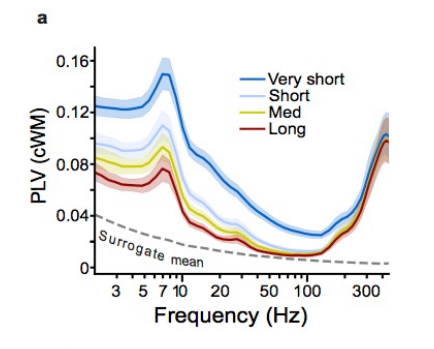
\includegraphics[width=0.3\textwidth]{14_4.PNG}} 
    \subfigure[]{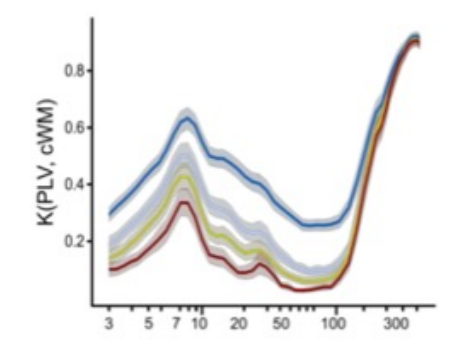
\includegraphics[width=0.3\textwidth]{14_5.PNG}}
\end{figure}
\begin{figure}[H]
    \centering
    \subfigure[]{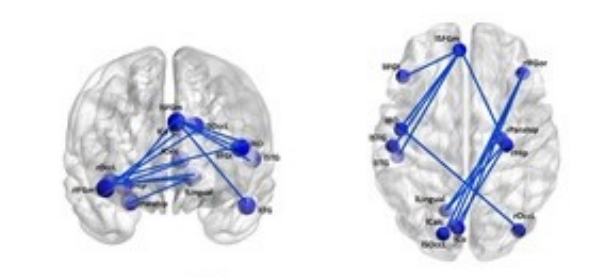
\includegraphics[width=0.4\textwidth]{14_6.PNG}} 
    \subfigure[]{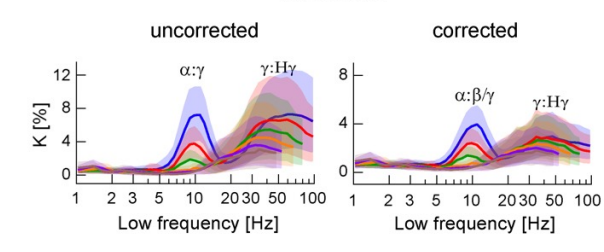
\includegraphics[width=0.4\textwidth]{14_7.PNG}}
\end{figure}
\subsection{Cross-frequency Coupling}
Brain activity can be observed at different time,frequency and spatial scales. Different oscillations can all together sum up on a single field activity.
\begin{figure}[H]
    \centering
    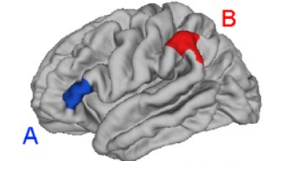
\includegraphics[scale=0.5]{14_8.PNG}
\end{figure}
Cross-frequency coupling is a communication mechanism between two different brain regions and is related to the concept of communication coherence, that says that the membrane potential and the LFP control the excitability of a cellular network. So, if the electrical fields of two regions oscillate with a constant time delay (in cross-connection), the probability of one stimulus to be transmitted from one area to the other is strongly connected to the time delay of these two excitability cycles of oscillations. Therefore, if the activity signal reaches the target region within its optimal excitability cycle the probability of communication is increased.\\
Neurons fire at higher firing frequencies than the field activity. So, through the field activity a spikes cannot be directly measured, it can only be assumed that the connectivity of slow oscillations is representing the excitability cycle or the CFC can be considered. 
\begin{figure}[H]
    \centering
    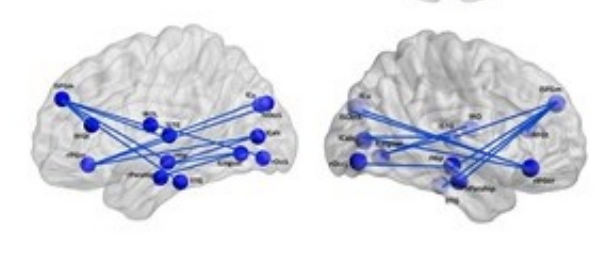
\includegraphics[scale=0.5]{14_9.PNG}
\end{figure}
The CFC attempts to measure the combination of phase and amplitude synchronization. Through this value, the probability of communication by looking at the phase of the slow oscillations in connection with the amplitude of the fast oscillations can be quantified. Every time the slow oscillations are synchronized there is an increase of amplitude in the high oscillations,and an increase of amplitude represents an increase in the firing activity.
The CFC can be measured in multiple ways:
\begin{itemize}
    \item \textbf{PAC (Phase-Amplitude Coupling)}, that looks at the correlation between synchronization of the slow rhythms and the co-increase of the amplitude oscillations.
    \begin{figure}[H]
    \centering
    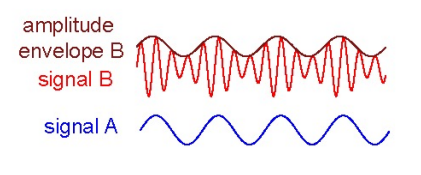
\includegraphics[scale=0.7]{14_10.PNG}
    \end{figure}
    \item \textbf{CFS (Cross-Frequency phase-phase Synchrony)} measures the coexistence of different oscillations and their relative space difference. So, it looks at the phase synchronization between two different rhythms.
    \begin{figure}[H]
    \centering
    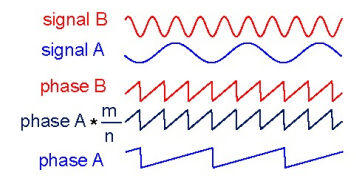
\includegraphics[scale=0.7]{14_11.PNG}
    \end{figure}
\end{itemize}

\subsection{PAC Algorithm}
Given to signals A and B recorded at two different sites of the brain:
\begin{enumerate}
    \item Filter A in a LF range (2 Hz) with the complex Morlet, so that the phase time series can be extracted.
    \item Filter B in a HF range (120 Hz) with the complex Morlet.
    \item To match together the two complex time series that have been found, the envelope from the filtered B is extracted (because we want to look at the amplitude increase that means that the local neurons under our probe are actively doing something).\\
    Now a phase-time series and an amplitude-time series that exists at the same time are obtained, so the PAC can be computed. But also the amplitude envelop contains spurious noise and needs to be filtered. It can be done with the same LF filter used for signal A.
    In this way specific amplitude modulation is considered, that exist in the same frequency range of the slow oscillations, so the noisy fast oscillations are being discarded.
    \item Compute PLV, but instead of doing it between two different channels withing the same band, the phase of 1 and the phase of 3 are used. In this way, the phase synchronization between two different regions and two different frequency bands can be observed, by looking at how the phase of slow oscillations modulate the amplitude increase.
\end{enumerate}
\begin{figure}[H]
    \centering
    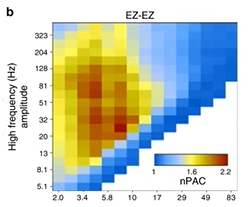
\includegraphics[scale=0.9]{14_12.PNG}
\end{figure}
If the algorithm is repeated for different pairs of frequency this plot can be built, where on the axes there are the low and the high frequency ranges. Each element represents the average of phase-amplitude coupling. There aren't elements in a part of the matrix because the phase modulation of the high frequency with the amplitude modulation of the slow frequency is not looked at, because that will be physiologically impossible.\\
So, this matrix shows how the different rhythms interact to each other into a complex network, and  allows to quantify how much the phase of one channel changes the amplitude of another channel. For example, it's well described the phase-amplitude coupling between theta and gamma mostly in the hippocampus.\\
What does an increase in PLV or PAC mean from a physiological point of view? Literature suggest that some increase in synchronization can be representative of neuro-degenerative process or pathological states (like epilepsy). An increase in phase synchronization of the theta band is linked to the successfully recall of memory from a memory task.
\subsection{Interaction Metrics: a list}
\subsubsection{Coherence}
Coherence is the ratio between the cross-spectrum and the product of the auto-spectra of the two signals. It represents linear spectral correlations between the two signals, so it cannot capture correlations that are not linear. It's sensitive to mixing factors (volume conduction), hidden sources (bivariate method) and common reference problems. An increase in coherence might either represent an increase in phase coherence or in amplitude correlation: these two elements cannot be separated just looking at this value.\\
This value allows a bivariate analysis, in whicb the correlation between two regions, A and B is computed. The problem is that between them also spurious connections are present, and not only significant ones.
\subsubsection{Partial Coherence}
The first attempt to expand the bivariate analysis has been the addition of a third channel to the estimation of coherence. The problem is that this method is very sensitive to SNR: if SNR isn't uniform in the 3 nodes a stronger partial coherence can be estimated in the wrong side of the network.
Furthermore, directional connectivity cannot be distinguished.
\subsubsection{Granger Causality}
It's useful for understanding directional communication. It's based on the estimation of an Auto-Regressive model and it only measures the linear dependency between two variables. Its value is comprised between 0 and 1.
It's based on the state that if the outcome of a variable X can be easily predicted by introducing prior knowledge of X and Y, this means that Y drives X.
This is not a real causality, but in some way it gives a directional information a bit larger than PLV.\\
However, in this algorithm there is an increase in the complexity in the estimation of the parameters.
\subsubsection{Multivariate Methods}
The majority of them rely on an Auto-Regressive models. The AR coefficients are derived such that the corresponding linear combination of the past values of the signal provides the best possible (in least squares sense) linear prediction of the current value. In practice, the MVAR method reduces to a method for estimating these coefficients and using them to compute various interaction measures. The solution of MVAR outputs a linear time-invariant system (LTI) which imposes limitations when applied to an obvious non linear system such as the human brain. Additionally, LTI imposes that the pdf of LTI output would be Gaussian.\\
Keep in mind that if the original data are passed through a temporal convolution filter, in most cases they will not follow an AR model because of the moving average term introduce by such filtering.
\subsubsection{Partial Directed Coherence and Direct Transfer Function}
They are based on the estimation of a Multivariate Auto Regressive model with the same criteria applied in the Granger Causality estimation.\\
As all the methods based on model fitting, the efficiency of these methods is strictly connected on the selection of initial parameters. This indeed boils down to the decision of the optimal model order and epoch length.\\
Causality estimated by means of GC, PDC and DTF is meaningful only in statistical sense, because their computation depends completely on an estimation of the model parameters. Also pre-processing steps can lead to very different results and interpretations.
\subsubsection{Mutual Information}
Can be very interesting to look at Mutual Information referred to spike analysis. This because an increase of that MI is an increase in communicability, instead in local field side is very complex to interpret. The problem with this type of metric is the computational cost.



